\documentclass[tikz, preview]{standalone}

\usepackage{amsfonts, amsthm, amssymb, amsmath, stmaryrd, etoolbox}
\usepackage{tikz}
\usepackage[all,2cell]{xy}
\usetikzlibrary{matrix,arrows,shapes,decorations.markings,decorations.pathreplacing}
\definecolor{rewritecolor}{rgb}{0,.9,1}
\tikzset{rewritenode/.style={shape=circle,fill=rewritecolor,scale=0.25,font=\Huge}}
\tikzset{RWopen/.style={shape=circle,draw=black,fill=white,scale=0.5,font=\Huge}}
\tikzset{RWclosed/.style={shape=circle,fill=black,scale=0.5,font=\Huge}}
\tikzset{CDnode/.style={shape=circle,fill=white,scale=.5}}
\tikzset{zxgreen/.style={shape=circle,draw,thick,fill=green}}
\tikzset{zxred/.style={shape=circle,draw,thick,fill=red}}
\tikzset{zxyellow/.style={shape=rectangle,draw,thick,fill=yellow}}
\tikzset{zxdiamond/.style={shape=diamond,fill=black,inner sep=2.75}}
\tikzset{zxopen/.style={shape=circle,draw,thick,inner sep=2pt}}
\tikzset{->-/.style={decoration={markings,mark=at position .5 with {\arrow{>}}},postaction={decorate}}}
\tikzset{->-pos/.style={decoration={
			markings,
			mark=at position #1 with {\arrow{>}}},postaction={decorate}}}


\begin{document}
\[
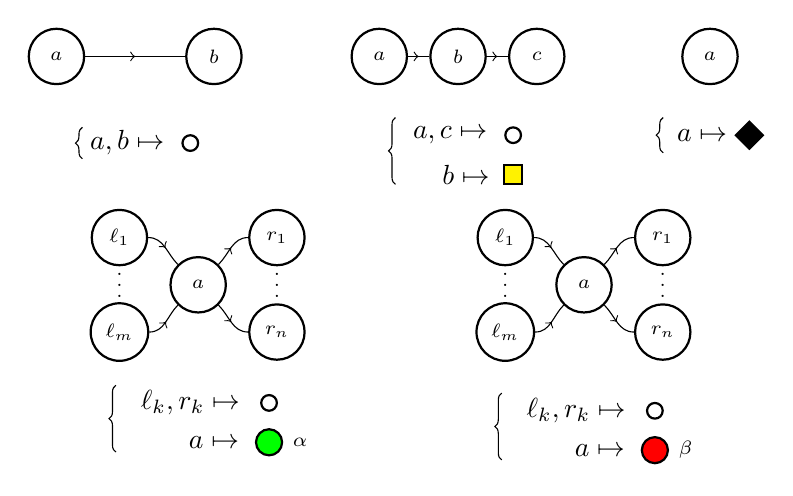
\begin{tikzpicture}
%
% WIRE
%
\begin{scope}[shift={(-1.8,6.1)}]
\begin{scope}[shift={(-1,0)}]
\node [circle,draw,thick,minimum size=20pt] (a) at (0,0) {\scriptsize $a$};
\node [circle,draw,thick,minimum size=20pt] (b) at (2,0) {\scriptsize $b$};
%
\draw [->-] (a) to (b);
\end{scope}
\begin{scope}[shift={(-0.1,-1.1)}]
\node at (0,0) {$a,b \mapsto$};
\node [zxopen] at (0.8,0) {};
\node (1) at (-0.5,0.2) {};
\node (2) at (-0.5,-0.2) {};
\draw [decoration={brace,mirror,raise=2pt},decorate] (1.center) -- (2.center); 	
\end{scope}
\end{scope}
%
% GREEN SPIDER
%
\begin{scope}[shift={(-1,3.2)}]
\begin{scope}[shift={(0,0)}]
\node [circle,draw,thick,minimum size=20pt] (a) at (0,0) {\scriptsize $a$}; 
\node [circle,draw,thick,minimum size=20pt] (1l) at (-1,0.6) {\scriptsize $\ell_1$};
\node [circle,draw,thick,minimum size=20pt] (m) at (-1,-0.6) {\scriptsize $\ell_m$};
\node at (-1,0.1) {\scriptsize $\vdots$};
\node [circle,draw,thick,minimum size=20pt] (1r) at (1,0.6) {\scriptsize $r_1$};
\node [circle,draw,thick,minimum size=20pt] (n) at (1,-0.6) {\scriptsize $r_n$};
\node at (1,0.1) {\scriptsize $\vdots$};
%
\draw [->-] (1l) to [out=0,in=135] (a);
\draw [->-] (m) to [out=0,in=-135] (a);
\draw [->-] (a) to [out=45,in=180] (1r);
\draw [->-] (a) to[out=-45,in=180] (n);
\end{scope}
\begin{scope}[shift={(-0.1,-1.5)}]
\node at (0,0) {$\ell_k, r_k \mapsto$};
\node at (0.3,-0.5) {$a \mapsto$};
\node [zxopen] at (1,0) {};
\node [zxgreen,label={[label distance=0pt]0:\scriptsize $\alpha$}] (3) at (1,-0.5) {};
\node (1) at (-0.75,0.1) {};
\node (2) at (-0.75,-0.5) {};
\draw [decoration={brace,mirror,raise=2pt},decorate] (1.north west) -- (2.south west); 	
\end{scope}
\end{scope}
%
% RED SPIDER
%
\begin{scope}[shift={(3.9,3.2)}]
\begin{scope}[shift={(0,0)}]
\node [circle,draw,thick,minimum size=20pt] (a) at (0,0) {\scriptsize $a$}; 
\node [circle,draw,thick,minimum size=20pt] (1l) at (-1,0.6) {\scriptsize $\ell_1$};
\node [circle,draw,thick,minimum size=20pt] (m) at (-1,-0.6) {\scriptsize $\ell_m$};
\node at (-1,0.1) {\scriptsize $\vdots$};
\node [circle,draw,thick,minimum size=20pt] (1r) at (1,0.6) {\scriptsize $r_1$};
\node [circle,draw,thick,minimum size=20pt] (n) at (1,-0.6) {\scriptsize $r_n$};
\node at (1,0.1) {\scriptsize $\vdots$};
%
\draw [->-] (1l) to [out=0,in=135] (a);
\draw [->-] (m) to [out=0,in=-135] (a);
\draw [->-] (a) to [out=45,in=180] (1r);
\draw [->-] (a) to [out=-45,in=180] (n);
\end{scope}
\begin{scope}[shift={(-0.1,-1.6)}]
\node at (0,0) {$\ell_k, r_k \mapsto$};
\node at (0.3,-0.5) {$a \mapsto$};
\node [zxopen] at (1,0) {};
\node [zxred,label={[label distance=0pt]0:\scriptsize $\beta$}] (3) at (1,-0.5) {};
\node (1) at (-0.75,0.1) {};
\node (2) at (-0.75,-0.5) {};
\draw [decoration={brace,mirror,raise=2pt},decorate] (1.north west) -- (2.south west); 	
\end{scope}
\end{scope}
%
% HADAMARD
%
\begin{scope}[shift={(2.3,6.1)}]
\begin{scope}[shift={(-1,0)}]
\node [circle,draw,thick,minimum size=20pt] (a) at (0,0) {\scriptsize $a$};
\node [circle,draw,thick,minimum size=20pt] (b) at (1,0) {\scriptsize $b$};
\node [circle,draw,thick,minimum size=20pt] (c) at (2,0) {\scriptsize $c$};
%
\draw [->-] (a) to (b);
\draw [->-] (b) to (c);
\end{scope}
\begin{scope}[shift={(-0.1,-1)}]
\node at (0,0) {$a,c \mapsto$};
\node at (0.2,-0.5) {$b \mapsto$};
\node [zxopen] at (0.8,0) {};
\node [zxyellow] (3) at (0.8,-0.5) {};
\node (1) at (-0.5,0.1) {};
\node (2) at (-0.5,-0.5) {};
\draw [decoration={brace,mirror,raise=2pt},decorate] (1.north west) -- (2.south west); 	
\end{scope}
\end{scope}
%
% DIAMOND
%
\begin{scope}[shift={(5.5,6.1)}]
\begin{scope}[shift={(0,0)}]
\node [circle,draw,thick,minimum size=20pt] (a) at (0,0) {\scriptsize $a$};
\end{scope}
\begin{scope}[shift={(-0.1,-1)}]
\node at (0,0) {$a \mapsto$};
\node (1) at (-0.3,0.1) {};
\node (2) at (-0.3,-0.1) {};
\node [zxdiamond] at (0.6,0) {};
\draw [decoration={brace,mirror,raise=2pt},decorate] (1.north west) -- (2.south west); 	
\end{scope}
\end{scope}
\end{tikzpicture}
\]
\end{document}
